\documentclass{article}
\usepackage{fullpage,graphicx}
\usepackage{amsmath,amsfonts,amsthm,amssymb,multirow}
\usepackage{algorithmic,comment,hyperref}
\usepackage[ruled,vlined,commentsnumbered,titlenotnumbered]{algorithm2e}
\usepackage{tikz}
\usetikzlibrary{decorations.pathreplacing}
\usetikzlibrary{shapes,positioning}
\newcommand{\expecting}[1]{\noindent\textbf{[We are expecting: #1]}}
\newcommand{\pts}[1]{\textbf{(#1 pt.)}}
\newcommand{\hint}[1]{\noindent\textbf{[HINT: #1]}}


\begin{document}
\noindent
CS 161 \hfill \textbf{Problem Set 7} \newline 
{Autumn 2017} \hfill \textbf{Due:} Friday December 1, 2017, at 3pm on Gradescope

\noindent
\rule{\linewidth}{0.4pt}

\section*{Exercises}
Exercises should be completed \textbf{on your own.}  

\noindent
\rule{\linewidth}{0.4pt}

\begin{enumerate}
\item \pts{2} Consider the graph $G$ below. 
\begin{center}
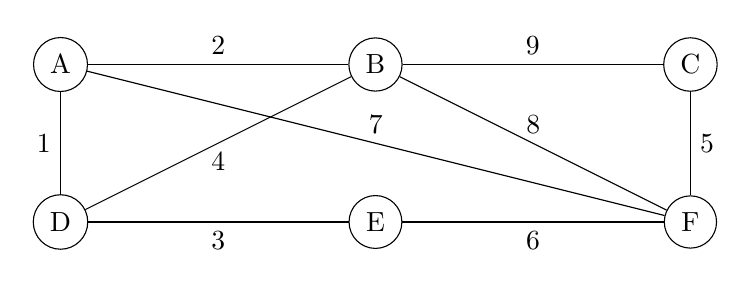
\begin{tikzpicture}[xscale=4,yscale=2]
\node[draw,circle](A) at (0,0) {A};
\node[draw,circle](B) at (1,0) {B};
\node[draw,circle](C) at (2,0) {C};
\node[draw,circle](D) at (0,-1) {D};
\node[draw,circle](E) at (1,-1) {E};
\node[draw,circle](F) at (2,-1) {F};
\draw (A) to node[left]{1} (D);
\draw (A) to node[above]{2} (B);
\draw (D) to node[below]{3} (E);
\draw (D) to node[below]{4} (B);
\draw (A) to node[above]{7} (F);
\draw (F) to node[below]{6} (E);
\draw (C) to node[right]{5} (F);
\draw (B) to node[above]{8} (F);
\draw (B) to node[above]{9} (C);
\end{tikzpicture}
\end{center}
\begin{enumerate}
\item \pts{1} What MST does Prim's algorithm return?  In what order does Prim's algorithm add edges to the MST when started from vertex $C$?

\item \pts{1} What MST does Kruskal's algorithm return? In what order does Kruskal's algorithm add edges to the MST?

\end{enumerate}
\expecting{For both, just a list of edges.  No justification is required.}


\vspace{1cm}
\item \pts{4} At a Thanksgiving dinner, there are $n$ food items $f_0,\ldots, f_{n-1}$.  Each food item has a tastiness $t_i > 0$ (measured in units of deliciousness per ounce) and a quantity $q_i > 0$ (measured in ounces).  There are $q_i$ ounces of food $f_i$ available to you, and for any real number $x \in [0,q_i]$, the total deliciousness that you derive from eating $x$ ounces of food $f_i$ is $x \cdot t_i$.  (Notice that $x$ here doesn't have to be an integer). 

Unfortunately, you only have capacity for $Q$ ounces of food in your belly, and you would like to maximize deliciousness subject to this constraint.  

\begin{enumerate}
\item \pts{2} Design a greedy algorithm which takes as input the tuples $(f_i, t_i, q_i)$, and outputs tuples $(f_i, x_i)$ so that $0 \leq x_i \leq q_i$, $\sum_i x_i \leq Q$, and $\sum_i x_i t_i$ is as large as possible.  Your algorithm should take time $O(n\log(n))$.

\expecting{Pseudocode and a short English explanation. }

\item \pts{2} Fill in the inductive step below to prove that your algorithm is correct.

\begin{itemize}
\item \textbf{Inductive hypothesis:} After making the $t$'th greedy choice, there is an optimal solution that extends the solution that the algorithm has constructed so far.
\item \textbf{Base case:} Any optimal solution extends the empty solution, so the inductive hypothesis holds for $t=0$.
\item \textbf{Inductive step:} \em (you fill in) \em
\item \textbf{Conclusion:} At the end of the algorithm, the algorithm returns an set $S^*$ of tuples $(f_i,x_i)$ so that $\sum_i x_i = Q$.  Thus, there is no solution extending $S^*$ other than $S^*$ itself.  Thus, the inductive hypothesis implies that $S^*$ is optimal.
\end{itemize}
\end{enumerate}

\end{enumerate}
\vfill
\noindent
\rule{\linewidth}{0.4pt}
\newpage
\section*{Problems}
You may talk with your fellow CS161-ers about the problems.  However:
\begin{itemize}
	\item Try the problems on your own \em before \em collaborating.
	\item Write up your answers yourself, in your own words.   You should never share your typed-up solutions with your collaborators.
	\item If you collaborated, list the names of the students you collaborated with at the beginning of each problem.
\end{itemize}

\noindent
\rule{\linewidth}{0.4pt}


\begin{enumerate}

\item\pts{6} Consider the problem of \textbf{making change.} Suppose that coins come in denominations $P = \{p_0,\ldots,p_m\}$ cents (for example, in the US, this would be $P = \{1,5,10,25\}$, corresponding to pennies, nickels, dimes, and quarters).  Given $n$ cents (where $n$ is a non-negative integer), you would like to find the way to represent $n$ using the fewest coins possible.  For example, in the US system, $55$ cents is minimally represented using three coins, two quarters and a nickel.

\begin{enumerate}
\item\pts{3} Suppose that the denominations are $P = \{1,10,25\}$ (aka, the US ran out of nickels).  Your friend uses the following greedy strategy for making change:

\begin{algorithm}[h]
\KwIn{ $n$ and $P$ }
coins $= [\,]$\;
\While{ $n > 0$ }
{
	$p^* \gets \max \{ p \in P \,:\, p \leq n \}$\;
	$n = n - p^*$\;
	coins.append($p^*$) \;
}
\Return{coins}
\caption{makeChange$(n)$}
\end{algorithm}
Your friend acknowledges that this won't work for general $P$ (for example if $P = \{2\}$ then we simply can't make any odd $n$), but claims that for this particular $P$ it does work.   
That is, your friend claims that this algorithm will always return a way to make $n$ out of the denominations in $P$ with the fewest coins possible. 

Is your friend correct for $P = \{1,10,25\}$?

\expecting{Your answer, and either a proof or a counterexample.  
If you do a proof by induction, make sure to explicitly state your inductive hypothesis, base case, inductive step, and conclusion.}

\item\pts{3}  Your friend says that additionally their algorithm should work for any $P$ of the form $P = \{1,2,4,8,\ldots, 2^s\}$.

Is your friend correct for $P = \{1,2,4,\ldots, 2^s\}$?

\expecting{Your answer, and either a proof or a counterexample.
If you do a proof by induction, make sure to explicitly state your inductive hypothesis, base case, inductive step, and conclusion.}

\end{enumerate}


\newpage
\item \pts{7}
On Thanksgiving day, you arrive on an island with $n$ turkeys.  You've already had thanksgiving dinner
(and maybe you prefer tofurkey anyway),
so you don't want to eat the turkeys; but you do want to wish them all a Happy Thanksgiving.  However, the turkeys each have very different sleep schedules.  Turkey $i$ is awake only in a single closed interval $[a_i,b_i]$.  Your plan is to stand in the center of the island and say loudly ``Happy Thanksgiving!" at certain times $t_1,\ldots, t_m$.  Any turkey who is awake at one of the times $t_j$ will hear the message.  It's okay if a turkey hears the message more than once, but you want to be sure that every turkey hears the message at least once.

\begin{enumerate}
\item \pts{3} Design a greedy algorithm which takes as input the list of intervals $[a_i,b_i]$ and outputs a list of times $t_1,\ldots,t_m$ so that $m$ is as small as possible and so that every turkey hears the message at least once.  Your algorithm should run in time $O(n\log(n))$.  

\expecting{Pseudocode and an English description of the main idea of your algorithm, as well as a short justification of the running time.}



\item \pts{4} Prove that your algorithm is correct.

\expecting{A proof by induction}


\end{enumerate} 

\vspace{1cm}
\item \pts{6}
Let $G$ be a connected weighted undirected graph.
In class, we defined a minimum spanning tree of $G$ as a spanning tree $T$ of $G$ which minimizes the quantity
\[ X = \sum_{e \in T} w_e, \]
where the sum is over all the edges in $T$, and $w_e$ is the weight of edge $e$.
Define a  ``minimum-maximum spanning tree" to be a spanning tree that minimizes the quantity
\[ Y = \max_{e \in T} w_e. \]
That is, a minimum-maximum spanning tree has the smallest maximum edge weight out of all possible spanning trees.
\begin{enumerate}

	\item \pts{4} Prove that a minimum spanning tree in a connected weighted undirected graph $G$ is always a minimum-maximum spanning tree for $G$.

	\expecting{ A short but formal proof. }
	\item \pts{2} Show that the converse to part (c) is not true.  That is, a minimum-maximum spanning tree is not necessarily a minimum spanning tree. 

	\expecting{ A counter-example, with an explanation of why it is a counter-example. }

	\item \pts{1 bonus} Give a deterministic $O(m)$ algorithm to find a minimum-maximum spanning tree in a connected weighted undirected graph $G$ with $n$ vertices and $m$ edges.

	\expecting{ Pseudocode, along with an English description of the idea of the algorithm, and an informal justification of correctness and running time.}
\end{enumerate}



\end{enumerate}
\end{document}
